% ====================================================================

% ====================================================================
\documentclass[article,paper=a4paper]{jlreq}

% jpreportパッケージの読み込み
\usepackage{jpreport}

% ページレイアウトの設定
\usepackage{geometry}
\usepackage{enumitem}
\geometry{
    top=25mm,
    bottom=25mm,
    left=25mm,
    right=25mm
}
% TikZライブラリ
\usetikzlibrary{
    patterns,
    calc,
    arrows,
    decorations,
    angles,
    shapes.geometric,
    fit,
    knots
}
% TikZ用のスタイル
\tikzset{
  every path/.style={
    black,
    line width=1pt
  },
  every node/.style={
    transform shape,
    knot crossing,
    inner sep=1.5pt
  }
}
% ハイパーリンクの設定
\usepackage[unicode]{hyperref}
\usepackage{bookmark}
\usepackage[nameinlink]{cleveref}

\hypersetup{
    colorlinks=true,
    linkcolor=black,
    urlcolor=blue,
    citecolor=blue,
    pdftitle=,
    pdfauthor=
}

% 数学演算子の定義


% cleveref用の日本語設定
\crefname{thm}{定理}{定理}
\crefname{lem}{補題}{補題}
\crefname{cor}{系}{系}
\crefname{ex}{例}{例}
\crefname{def}{定義}{定義}
\crefname{prop}{命題}{命題}
\crefname{prob}{問題}{問題}

% 色彩の定義
\definecolor{yukari}{RGB}{196, 163, 191}

% 文書情報
\title{応用数理1}
\author{akari0koutya}
\date{\today}

\begin{document}

% --- タイトル ------------------------------------------------------
\maketitle
\begin{abstract}
  グラフ理論，組合せ論の諸概念，結果及び手法について応用を交えて学ぶ。
\end{abstract}
\tableofcontents
%% 本文の内容をここに記述
% ====================================================================

\section{第1回(2026/04/15)}

\begin{dfn}
    \textbf{無向グラフ} $G$ とは、空でない有限集合 $V(G)$ と $V(G) \times V(G)$ の部分集合 $E(G)$ からなる組である。$V(G)$ の元を \textbf{頂点} と呼び、$E(G)$ の元を \textbf{辺} と呼ぶ。
\end{dfn}

\begin{figure}[htbp]
  \centering
  \begin{minipage}{0.45\textwidth}
    \centering
    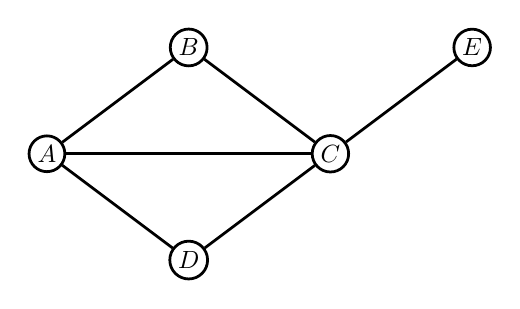
\begin{tikzpicture}[thick, scale=0.9]
    % 頂点
    \node[draw,circle] (A) at (0,0) {$A$};
    \node[draw,circle] (B) at (2,1.5) {$B$};
    \node[draw,circle] (C) at (4,0) {$C$};
    \node[draw,circle] (D) at (2,-1.5) {$D$};
    \node[draw,circle] (E) at (6,1.5) {$E$};

    % 辺（無向）
    \draw (A) -- (B);
    \draw (B) -- (C);
    \draw (C) -- (D);
    \draw (D) -- (A);
    \draw (A) -- (C);
    \draw (C) -- (E);
    \end{tikzpicture}
  \end{minipage}
  \begin{minipage}{0.45\textwidth}
    \centering
    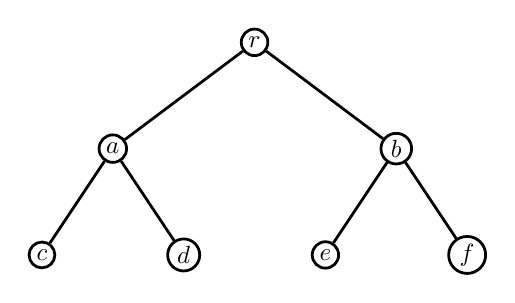
\begin{tikzpicture}[thick, scale=0.9]
    % 頂点
    \node[draw,circle] (R) at (0,0) {$r$};
    \node[draw,circle] (A) at (-2,-1.5) {$a$};
    \node[draw,circle] (B) at (2,-1.5) {$b$};
    \node[draw,circle] (C) at (-3,-3) {$c$};
    \node[draw,circle] (D) at (-1,-3) {$d$};
    \node[draw,circle] (E) at (1,-3) {$e$};
    \node[draw,circle] (F) at (3,-3) {$f$};

    % 辺
    \draw (R) -- (A);
    \draw (R) -- (B);
    \draw (A) -- (C);
    \draw (A) -- (D);
    \draw (B) -- (E);
    \draw (B) -- (F);
    \end{tikzpicture}
  \end{minipage}
  \caption{グラフの例}
\end{figure}

\begin{dfn}
  $G$ : 無向グラフ\\
  $G$ の頂点 $v$ に接続されている辺の数を $G$ の $v$ における\textbf{次数}と呼び、$\deg_G(v)$ で表す。
\end{dfn}

\begin{prop}
  \quad $G$ : 無向グラフ\par
  $\sum_{v \in V(G)} \deg_G(v) = 2|E(G)|$ が成り立つ。
\end{prop}

\begin{proof}
  各辺はちょうど2つの頂点に接続されているため、$\sum_{v \in V(G)} \deg_G(v)$ は $G$ の辺の数 $|E(G)|$ の2倍になる。
\end{proof}

\begin{cor}
  \quad $G$ : 無向グラフ\par
  $G$ の頂点の次数の和は偶数である。
\end{cor}

\begin{proof}
  $\sum_{v \in V(G)} \deg_G(v) = 2|E(G)|$ より、$\sum_{v \in V(G)} \deg_G(v)$ は偶数である。
\end{proof}

\begin{dfn}
  $G_1$, $G_2$ : 無向グラフ
  \begin{itemize}
    \item $G_1$ と $G_2$ が \textbf{同一} であるとは、$V(G_1) = V(G_2)$ かつ $E(G_1) = E(G_2)$ であることをいう。
    \item $G_1$ と $G_2$ が \textbf{同型} であるとは、全単射 $f: V(G_1) \to V(G_2)$ が存在し、任意の $u, v \in V(G_1)$ に対して、$uv \in E(G_1)$ であることと $f(u)f(v) \in E(G_2)$ であることが同値であることをいう。
  \end{itemize}
\end{dfn}

\begin{ex}
  \quad 以下のグラフ $G$ と $H$ は同型である。なぜなら、全単射 $f: V(G) \to V(H)$ を以下のように定義できるからである :
\[
A\mapsto u,\quad
B\mapsto q,\quad
C\mapsto s,\quad
D\mapsto p,\quad
E\mapsto t,\quad
F\mapsto r
\]
\end{ex}

\begin{figure}[htbp]
  \begin{minipage}{0.45\textwidth}
    \centering
    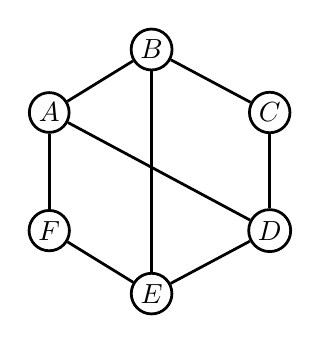
\begin{tikzpicture}[thick]

    %-------------------------
    % 左のグラフ G
    %-------------------------
    \node[draw,circle] (A) at (0,1.5) {$A$};
    \node[draw,circle] (B) at (1.3,2.3) {$B$};
    \node[draw,circle] (C) at (2.8,1.5) {$C$};
    \node[draw,circle] (D) at (2.8,0) {$D$};
    \node[draw,circle] (E) at (1.3,-0.8) {$E$};
    \node[draw,circle] (F) at (0,0) {$F$};

    \draw (A) -- (B);
    \draw (B) -- (C);
    \draw (C) -- (D);
    \draw (D) -- (E);
    \draw (E) -- (F);
    \draw (F) -- (A);
    \draw (A) -- (D);
    \draw (B) -- (E);

    \node at (1.4,-1.6) {$G$};
    \end{tikzpicture}
  \end{minipage}
  \begin{minipage}{0.45\textwidth}
    \centering
    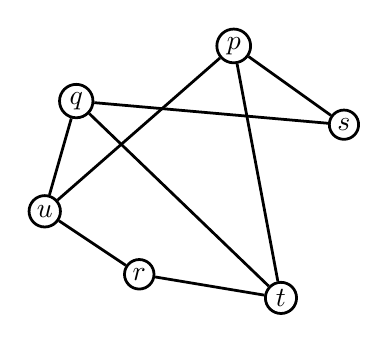
\begin{tikzpicture}[thick]
    %-------------------------
    %rightのグラフ H
    %-------------------------
    \node[draw,circle] (p) at (8.8,2.2) {$p$};
    \node[draw,circle] (q) at (6.8,1.5) {$q$};
    \node[draw,circle] (r) at (7.6,-0.7) {$r$};
    \node[draw,circle] (s) at (10.2,1.2) {$s$};
    \node[draw,circle] (t) at (9.4,-1.0) {$t$};
    \node[draw,circle] (u) at (6.4,0.1) {$u$};

    \draw (u) -- (q);
    \draw (q) -- (s);
    \draw (s) -- (p);
    \draw (p) -- (t);
    \draw (t) -- (r);
    \draw (r) -- (u);
    \draw (u) -- (p);
    \draw (q) -- (t);

    \node at (8.3,-1.8) {$H$};

    \end{tikzpicture}
  \end{minipage}
  \caption{同型グラフの例}
\end{figure}

\begin{dfn}
  \quad $G$, $H$ : 無向グラフ
  \begin{itemize}
    \item $V(H) \subseteq V(G)$ かつ $E(H) \subseteq E(G)$ であるとき、$H$ は $G$ の \textbf{部分グラフ} であるといい、$H \subseteq G$ と表す。
    \item 上でさらに $V(H) = V(G)$ であるとき、$H$ は $G$ の \textbf{全域部分グラフ} であるという。
    \item $S \subseteq V(G)$ とし、$V(\langle S \rangle_G) = S$ かつ $E(\langle S \rangle_G) = \{uv \in E(G) \mid u, v \in S\}$ と定めるとき、$\langle S \rangle_G$ を $G$ の $S$ による \textbf{誘導部分グラフ} という。
  \end{itemize}
\end{dfn}

\begin{figure}[htbp]
\centering

%---------------------------------
% 元のグラフ
%---------------------------------
\begin{minipage}{0.3\textwidth}
\centering
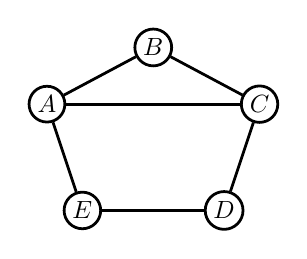
\begin{tikzpicture}[thick,scale=0.9]
    % 頂点
    \node[draw,circle] (A) at (0,1.5) {$A$};
    \node[draw,circle] (B) at (1.5,2.3) {$B$};
    \node[draw,circle] (C) at (3,1.5) {$C$};
    \node[draw,circle] (D) at (2.5,0) {$D$};
    \node[draw,circle] (E) at (0.5,0) {$E$};

    % 辺
    \draw (A) -- (B);
    \draw (B) -- (C);
    \draw (C) -- (D);
    \draw (D) -- (E);
    \draw (E) -- (A);
    \draw (A) -- (C);
\end{tikzpicture}

\smallskip

元のグラフ $G$
\end{minipage}
\hfill
%---------------------------------
% 全域部分グラフ
%---------------------------------
\begin{minipage}{0.3\textwidth}
\centering
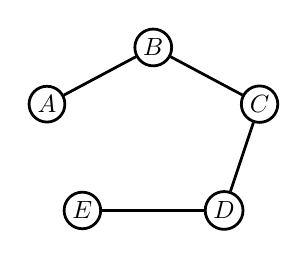
\begin{tikzpicture}[thick,scale=0.9]
    % 頂点
    \node[draw,circle] (A) at (0,1.5) {$A$};
    \node[draw,circle] (B) at (1.5,2.3) {$B$};
    \node[draw,circle] (C) at (3,1.5) {$C$};
    \node[draw,circle] (D) at (2.5,0) {$D$};
    \node[draw,circle] (E) at (0.5,0) {$E$};

    % 辺（頂点は全部残し、辺だけ減らす）
    \draw (A) -- (B);
    \draw (B) -- (C);
    \draw (C) -- (D);
    \draw (D) -- (E);
\end{tikzpicture}

\smallskip

全域部分グラフ
\end{minipage}
\hfill
%---------------------------------
% 誘導部分グラフ
%---------------------------------
\begin{minipage}{0.3\textwidth}
\centering
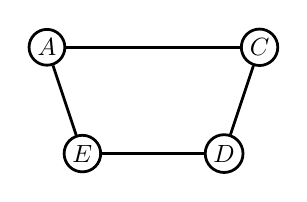
\begin{tikzpicture}[thick,scale=0.9]
    % 頂点集合 {A,C,D,E}
    \node[draw,circle] (A) at (0,1.5) {$A$};
    \node[draw,circle] (C) at (3,1.5) {$C$};
    \node[draw,circle] (D) at (2.5,0) {$D$};
    \node[draw,circle] (E) at (0.5,0) {$E$};

    % 誘導部分グラフなので、この頂点間に元のグラフで存在する辺をすべて入れる
    \draw (A) -- (C);
    \draw (C) -- (D);
    \draw (D) -- (E);
    \draw (E) -- (A);
\end{tikzpicture}

\smallskip

誘導部分グラフ
\end{minipage}

\caption{グラフ $G$ と、その全域部分グラフおよび誘導部分グラフの例}
\label{fig:graph-subgraphs}
\end{figure}

\end{document}